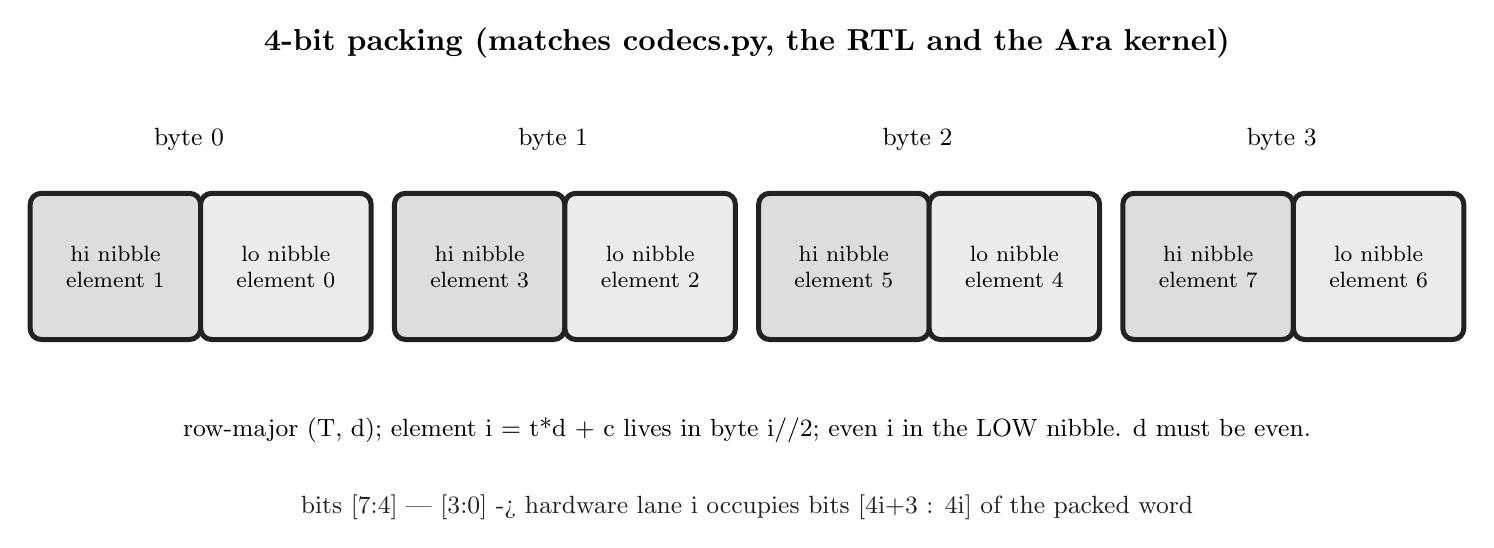
\begin{tikzpicture}[line cap=round,line join=round]
\draw[rounded corners=4.0pt,line width=1.82pt,draw={rgb,255:red,34;green,34;blue,34},fill={rgb,255:red,221;green,221;blue,221}] (0.291in,1.136in) rectangle (1.143in,1.867in);
\draw[rounded corners=4.0pt,line width=1.82pt,draw={rgb,255:red,34;green,34;blue,34},fill={rgb,255:red,236;green,236;blue,236}] (1.143in,1.136in) rectangle (1.996in,1.867in);
\draw[rounded corners=4.0pt,line width=1.82pt,draw={rgb,255:red,34;green,34;blue,34},fill={rgb,255:red,221;green,221;blue,221}] (2.112in,1.136in) rectangle (2.964in,1.867in);
\draw[rounded corners=4.0pt,line width=1.82pt,draw={rgb,255:red,34;green,34;blue,34},fill={rgb,255:red,236;green,236;blue,236}] (2.964in,1.136in) rectangle (3.817in,1.867in);
\draw[rounded corners=4.0pt,line width=1.82pt,draw={rgb,255:red,34;green,34;blue,34},fill={rgb,255:red,221;green,221;blue,221}] (3.933in,1.136in) rectangle (4.786in,1.867in);
\draw[rounded corners=4.0pt,line width=1.82pt,draw={rgb,255:red,34;green,34;blue,34},fill={rgb,255:red,236;green,236;blue,236}] (4.786in,1.136in) rectangle (5.638in,1.867in);
\draw[rounded corners=4.0pt,line width=1.82pt,draw={rgb,255:red,34;green,34;blue,34},fill={rgb,255:red,221;green,221;blue,221}] (5.754in,1.136in) rectangle (6.607in,1.867in);
\draw[rounded corners=4.0pt,line width=1.82pt,draw={rgb,255:red,34;green,34;blue,34},fill={rgb,255:red,236;green,236;blue,236}] (6.607in,1.136in) rectangle (7.459in,1.867in);
\node[anchor=south,align=center,text={rgb,255:red,0;green,0;blue,0},font=\fontsize{11.0pt}{13.0pt}\selectfont\bfseries,inner sep=0pt] at (3.875in,2.541in) {4-bit packing (matches codecs.py, the RTL and the Ara kernel)};
\node[anchor=south,align=center,text={rgb,255:red,0;green,0;blue,0},font=\fontsize{9.0pt}{10.6pt}\selectfont,inner sep=0pt] at (1.085in,2.079in) {byte 0};
\node[align=center,text={rgb,255:red,0;green,0;blue,0},font=\fontsize{8.0pt}{9.4pt}\selectfont,inner sep=0pt] at (0.717in,1.502in) {hi nibble \\ element 1};
\node[align=center,text={rgb,255:red,0;green,0;blue,0},font=\fontsize{8.0pt}{9.4pt}\selectfont,inner sep=0pt] at (1.569in,1.502in) {lo nibble \\ element 0};
\node[anchor=south,align=center,text={rgb,255:red,0;green,0;blue,0},font=\fontsize{9.0pt}{10.6pt}\selectfont,inner sep=0pt] at (2.906in,2.079in) {byte 1};
\node[align=center,text={rgb,255:red,0;green,0;blue,0},font=\fontsize{8.0pt}{9.4pt}\selectfont,inner sep=0pt] at (2.538in,1.502in) {hi nibble \\ element 3};
\node[align=center,text={rgb,255:red,0;green,0;blue,0},font=\fontsize{8.0pt}{9.4pt}\selectfont,inner sep=0pt] at (3.391in,1.502in) {lo nibble \\ element 2};
\node[anchor=south,align=center,text={rgb,255:red,0;green,0;blue,0},font=\fontsize{9.0pt}{10.6pt}\selectfont,inner sep=0pt] at (4.728in,2.079in) {byte 2};
\node[align=center,text={rgb,255:red,0;green,0;blue,0},font=\fontsize{8.0pt}{9.4pt}\selectfont,inner sep=0pt] at (4.359in,1.502in) {hi nibble \\ element 5};
\node[align=center,text={rgb,255:red,0;green,0;blue,0},font=\fontsize{8.0pt}{9.4pt}\selectfont,inner sep=0pt] at (5.212in,1.502in) {lo nibble \\ element 4};
\node[anchor=south,align=center,text={rgb,255:red,0;green,0;blue,0},font=\fontsize{9.0pt}{10.6pt}\selectfont,inner sep=0pt] at (6.549in,2.079in) {byte 3};
\node[align=center,text={rgb,255:red,0;green,0;blue,0},font=\fontsize{8.0pt}{9.4pt}\selectfont,inner sep=0pt] at (6.181in,1.502in) {hi nibble \\ element 7};
\node[align=center,text={rgb,255:red,0;green,0;blue,0},font=\fontsize{8.0pt}{9.4pt}\selectfont,inner sep=0pt] at (7.033in,1.502in) {lo nibble \\ element 6};
\node[anchor=south,align=center,text={rgb,255:red,0;green,0;blue,0},font=\fontsize{9.0pt}{10.6pt}\selectfont,inner sep=0pt] at (3.875in,0.616in) {row-major (T, d); element i = t*d + c lives in byte i//2; even i in the LOW nibble.   d must be even.};
\node[anchor=south,align=center,text={rgb,255:red,34;green,34;blue,34},font=\fontsize{9.0pt}{10.6pt}\selectfont,inner sep=0pt] at (3.875in,0.231in) {bits [7:4] | [3:0]   ->   hardware lane i occupies bits [4i+3 : 4i] of the packed word};
\end{tikzpicture}
